\clearpage
\twocolumn[{%
\rqparent
\subsection{Size generalisation to 3B}
\label{app:rq10_size_generalisation}

\noindent\begin{minipage}[t]{0.485\textwidth}
\vspace{0pt}
\paragraph{Research Question.} \emph{Does a ranking that holds at 1.7B still hold one rung above it, at 3B?}

\paragraph{Setup.} We test whether the conclusions hold with a 3B reference. We compare the share of tasks above chance at 1.7B and at 3B, and DA-size against the 3B and the 1.7B final checkpoints on the same decisions. We use the six deep configurations trained to 3B at seed 1904 (scheme A at K $\in$ \{8, 15, 30, 50\}, scheme B at K $\in$ \{8, 15\}) and the same configurations at 90M--1.7B. Benchmark accuracy covers the tasks above chance at the proxy, at 1.7B and at 3B, the bBPB twins included (they exist for five of the six 3B models, all but K = 30). The share panel recomputes the Wilson rule at 1.7B and at 3B on the six configurations alone, over the runs that train the task's language (one to six runs per task). The DA panel gates the proxies and 1.7B with the gate of every seed-1904 run and 3B with the rule on the six 3B runs. Per-language BPB (14 languages, DCLM English and the mixture macro-average) is pooled separately. We pool the matching pairs over the tasks, with at least three pairs per task. The bands are 90 \% leave-one-family-out jackknife bands. The share panel shows the 15 benchmarks that have at least five tasks and whose share changes.
\end{minipage}\hfill
\begin{minipage}[t]{0.485\textwidth}
\vspace{0pt}
\begin{rqfinding}
\textbf{1. The 3B rung measures more than the reference but decides no differently.} On the same six families, it lifts the above-chance count from 607 to 772 of 927 tasks (+27 \%). On identical mono-axis decisions, DA-size stays at 0.49--0.54 in benchmark accuracy (bBPB twins pooled) and at 0.78--0.91 in per-language BPB, whichever the reference. (Figure~\ref{fig:app_rq10_size_generalisation}.)
\\
\\
\textbf{2. In benchmark accuracy no proxy predicts the 3B decision, the 1.7B reference included.} On the six families' gated benchmark tasks (the bBPB twins left out), DA-size $\rightarrow$ 3B is 0.48--0.53 mono-axis over 184--281 tasks and 0.48--0.53 multi-axis over 209--326.
\\
\\
\textbf{3. Without the bBPB twins the two references still agree.} On identical decisions without the twins, DA-size is 0.48--0.53 to 1.7B and 0.48--0.53 to 3B, mono-axis (per-task table of ).
\end{rqfinding}
\end{minipage}

\vspace{\baselineskip}
\noindent\begin{minipage}{\textwidth}
\centering
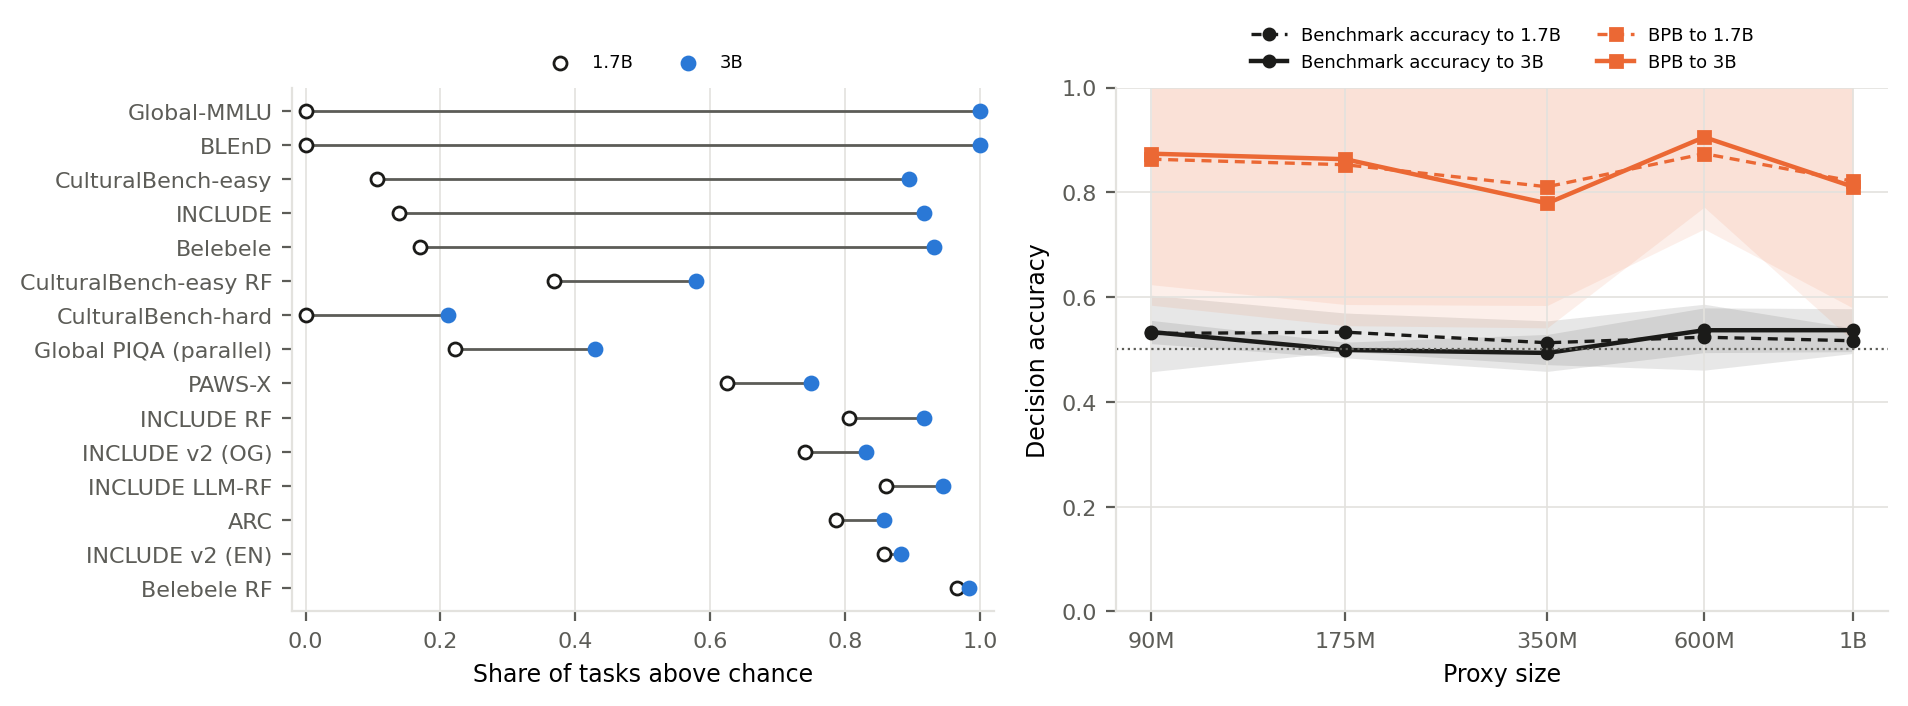
\includegraphics[width=\textwidth,height=0.36\textheight,keepaspectratio]{figures/app_rq10_size_generalisation.png}
% source: src/signal-and-noise/analysis/rq10_size_generalisation/pretraining/predictivity/gate_share_and_da_size_mono_axis_paper.png
\captionof{figure}{\textbf{The 3B rung measures more than the reference but decides no differently.} Left: for each benchmark with at least five tasks whose share moves, the share of its tasks above chance at 1.7B (open circles) and at 3B (filled circles). Right: DA-size of the proxies 90M--1B against the 3B final checkpoint (solid) and against the 1.7B final checkpoint (dashed), on benchmark accuracy (black) and on per-language bits per byte (orange). The bands are 90\% leave-one-family-out jackknife bands and the dotted line marks 0.5.}
\label{fig:app_rq10_size_generalisation}
\end{minipage}
}]

\begin{figure*}[p]
\centering
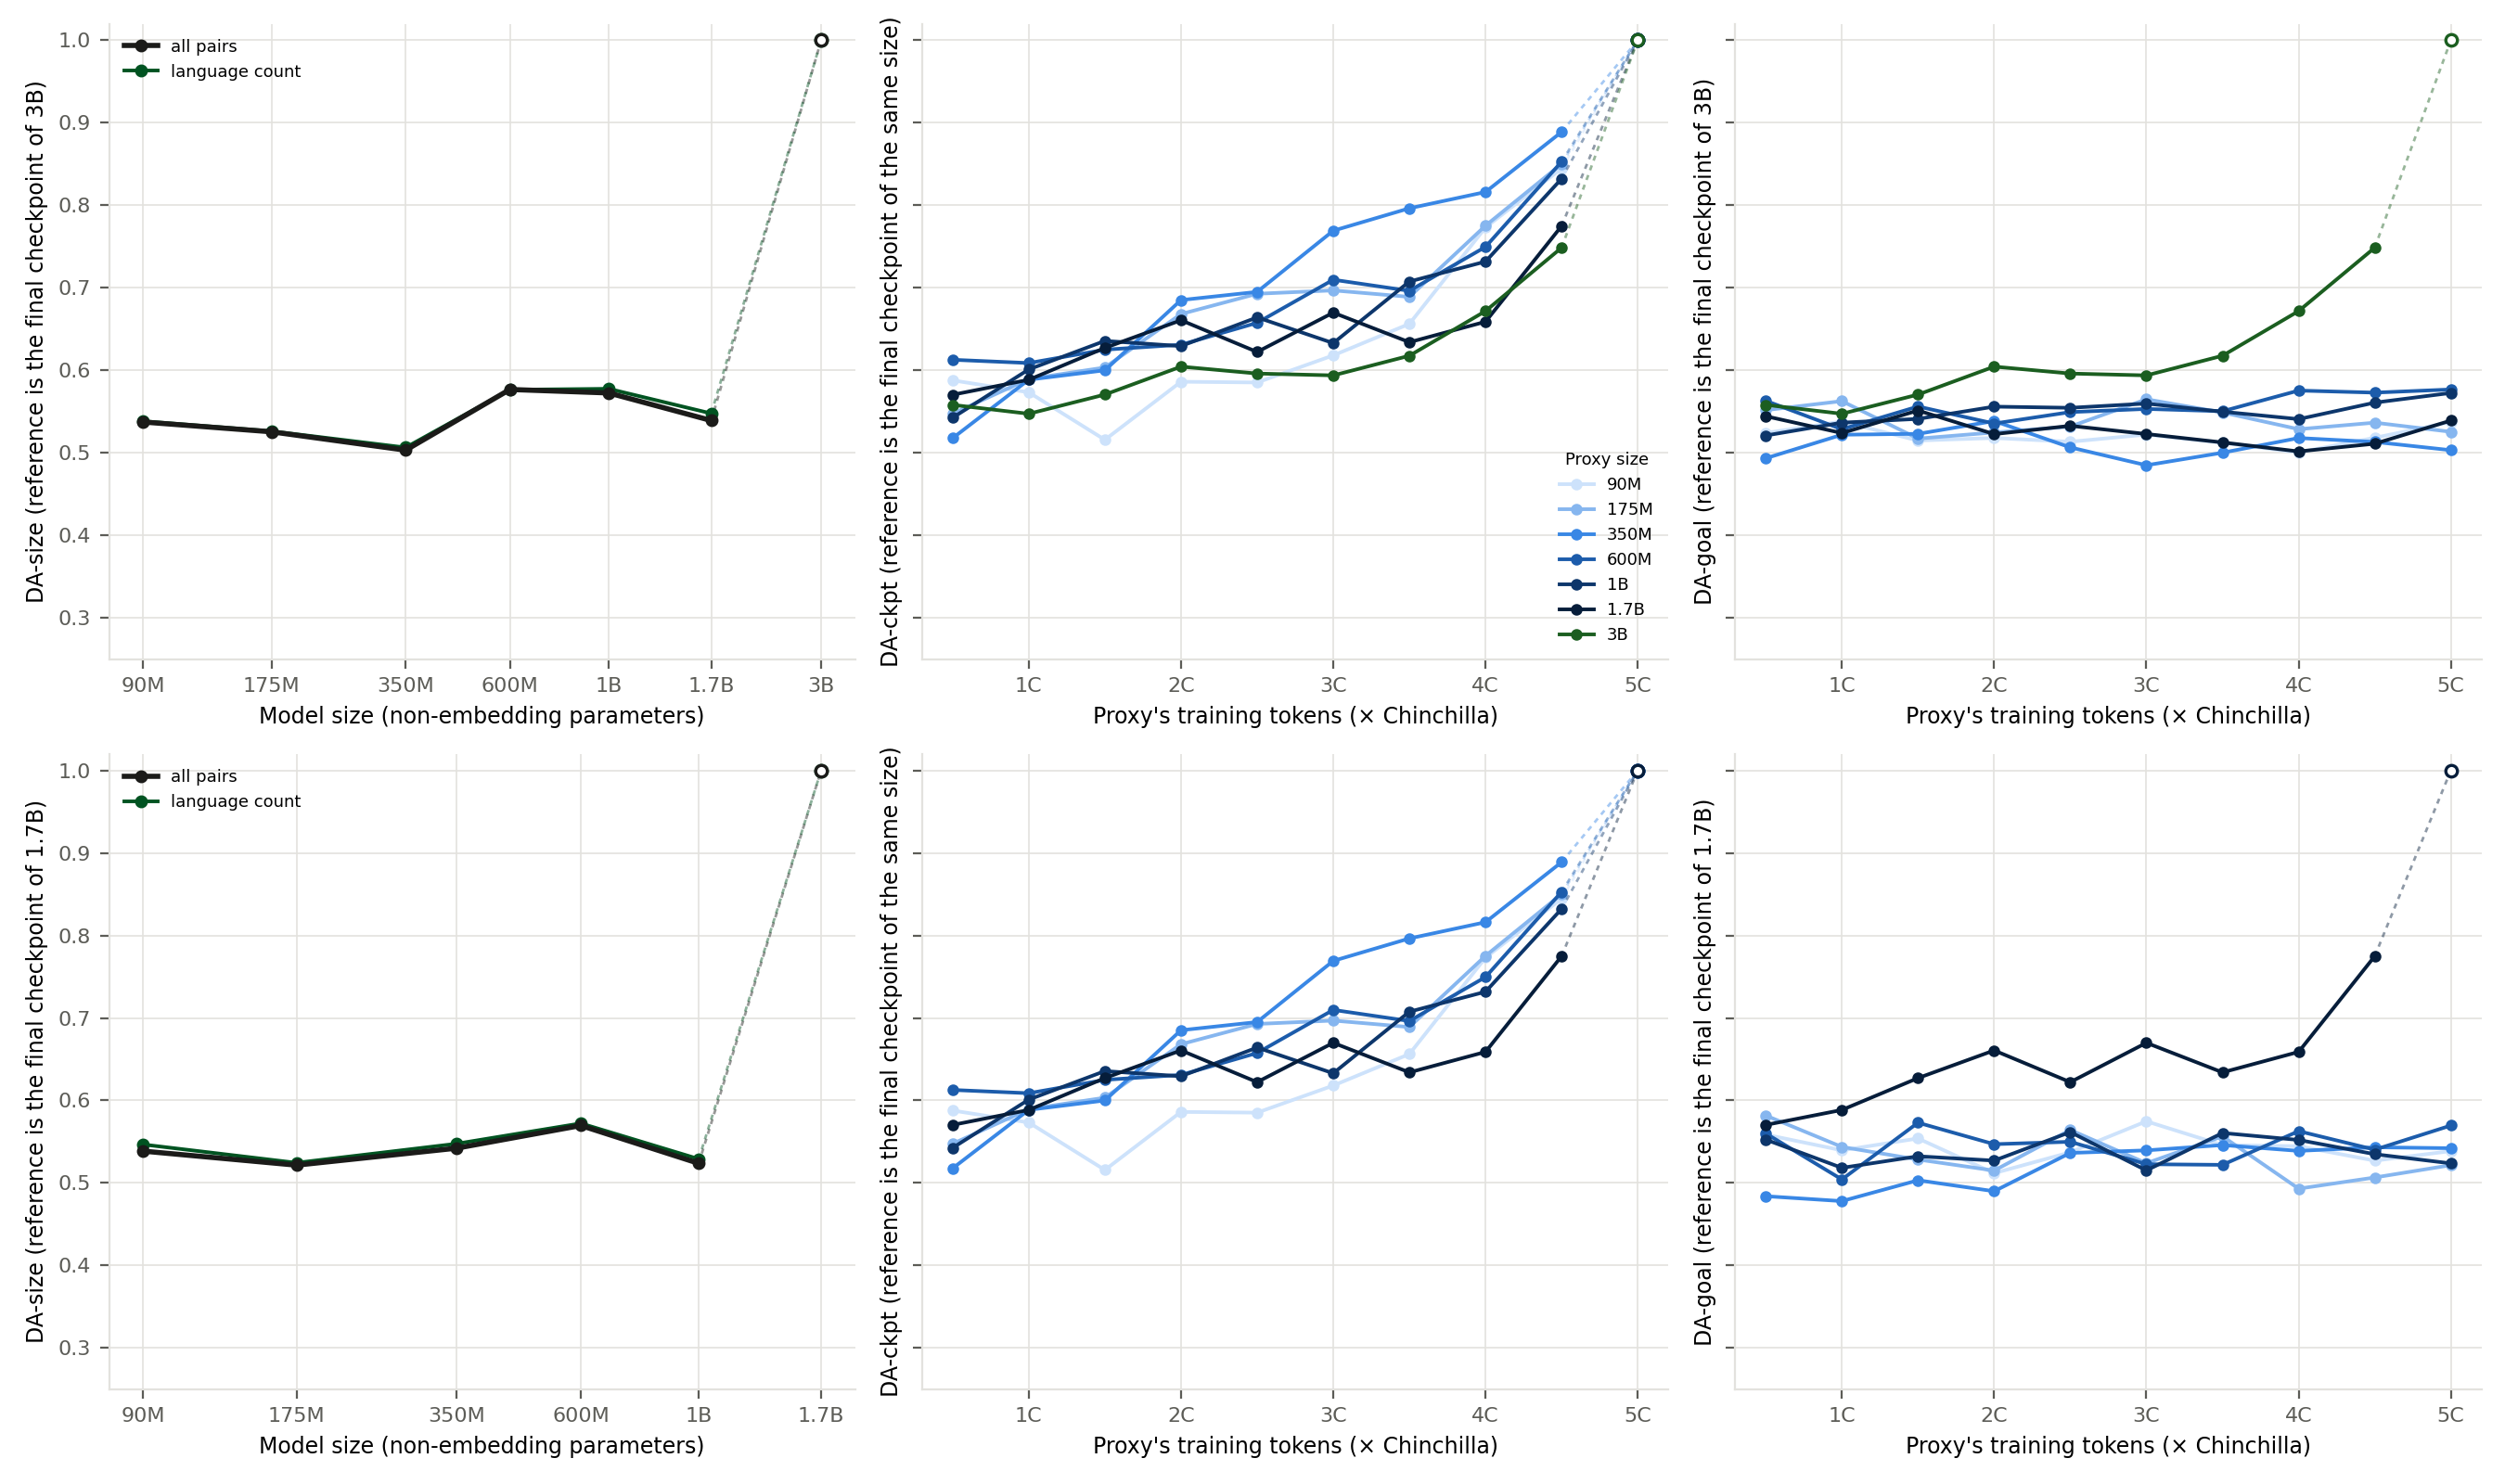
\includegraphics[width=\textwidth,height=0.8\textheight,keepaspectratio]{figures/rq2_3b_compare.png}
% source: documents/paper/figures/make_rq2_3b.py (not in make_rq_appendix.py's FIGURES: add it there before regenerating this page)
\caption{\textbf{A 3B reference ranks the proxies no better than the 1.7B one.} Figure~\ref{fig:rq2} on the six configurations trained at 3B (deep, scheme A at $K \in \{8, 15, 30, 50\}$, scheme B at $K \in \{8, 15\}$, seed 1904), against the final 3B checkpoint (top) and against the final 1.7B checkpoint (bottom). Both rows read the nine single-axis pairs of these configurations and the 553 tasks whose median DA-size or median DA-ckpt is at least 0.66 under both references (394 of them bBPB twins), so they differ in the reference alone. A task enters a point when it is above chance at the proxy and at the reference: 339--392 tasks per point against 3B, where the 3B model at $K=30$ has no bBPB twins, and 499--549 against 1.7B. \textbf{(a)} DA-size of the final checkpoint of each size. Only the number of languages has at least three pairs (seven), so the black line over all pairs nearly matches it, and the data-scheme line (two pairs) is dropped. \textbf{(b)} DA-ckpt against the final checkpoint of the same size, which does not depend on the reference. The 3B run stabilises last. \textbf{(c)} DA-goal of every checkpoint against the reference. Every proxy reads 0.48--0.58 against either reference, the 1.7B proxy included (0.50--0.55 against 3B), while the reference's own run rises to 0.75--0.77 at 4.5C.}
\label{fig:app_rq2_3b_compare}
\end{figure*}

